\documentclass[12pt]{article}
\usepackage[margin=1in]{geometry}
\usepackage{epsfig}
\usepackage{amsfonts}
\usepackage[mathcal]{euscript}
\usepackage[tbtags]{amsmath}
\usepackage{amssymb}
\usepackage{mathrsfs}
\usepackage{import}
\usepackage{hyperref}
%\usepackage{minted}
\usepackage{enumerate}
\usepackage{algorithm}
\usepackage{algorithmicx}
\usepackage[noend]{algpseudocode}

\renewcommand{\P}{\mathbb{P}}

\newcommand{\example}[3]{%
    \vspace{.15in}

    \noindent \textbf{Example~#1}\nopagebreak

    \noindent #2

    \noindent \textbf{Solution}: #3
}


\DeclareMathOperator*{\argmax}{\mathrm{argmax}}
\renewcommand{\P}{\mathbb{P}}
\newcommand{\bunderline}[2][4]{\underline{#2\mkern-#1mu}\mkern#1mu}
\newcommand{\phat}{\widehat{p}_X}
\newcommand{\uX}{{\bunderline{X}}}
\newcommand{\ux}{{\bunderline{x}}}
\newcommand{\uY}{{\bunderline{Y}}}
\newcommand{\uy}{{\bunderline{y}}}
\newcommand{\tp}{\widetilde{p}}

\title{The Ising model and Markov chain Monte Carlo}
\author{Ramesh Sridharan\thanks{Contact: \mbox{rameshvs@csail.mit.edu}}}
\date{}
\algrenewcommand\algorithmicrequire{\textbf{Inputs:}}
\begin{document}
    \maketitle
    These notes give a short description of the Ising model for images and an
    introduction to Metropolis-Hastings and Gibbs Markov Chain Monte Carlo (MCMC).
    These notes assume you're familiar with basic probability and graphical models.
    
    The notation here is borrowed from \emph{Introduction to Probability} by
    Bertsekas \& Tsitsiklis: random variables are represented with capital
    letters, values they take are represented with lowercase letters, $p_X$
    represents a probability distribution for random variable $X$, and $p_X(x)$
    represents the probability of value $x$ (according to $p_X$).
    \section{The Ising model}

    In many cases where we're interested in doing inference, we can't do
    it exactly. With such cases, we can approximate the true distribution using
    samples from it.  Let's look at a model where we need to use techniques
    like this: the \emph{Ising model}~\footnote{Technically, the Ising model
        refers to a model like the one described, but where each $X_i$ takes on
        values in $\{-1, +1\}$ instead of $\{0,1\}$. The model here is also
        frequently referred to as a Markov Random Field, or MRF, even though
        the term MRF is in fact more general. The standard Ising model (as
        described in physics) also doesn't have associated observations,
        but this usage is common enough in machine learning.}.

    The Ising model isn't the only one where sampling techniques like the ones
    we'll discuss are useful, and these techniques aren't the only way to do
    approximate inference here, but they provide a convenient story for
    illustrating both ideas.

    \subsection{Ising model for images}
    Suppose we have a binary image: that is, each pixel can either be 0 or 1.
    Let $X_i$ be a random variable with the value of pixel $i$, and let's say
    we have $n$ pixels. To save ourselves some writing, we'll use $\uX$ to
    represent the set $\{X_1, X_2, \ldots, X_n\}$. The Ising model says that
    the distribution for $\uX$ is:
    \begin{align}
        \label{eq:ising} p_\uX(\ux) &= \frac{1}{Z} \prod_{(i,j) \in E} \psi(x_i, x_j),
    \end{align}
    where
    \begin{itemize}
        \item $\psi(\cdot, \cdot)$ is an \emph{edge potential} that's usually chosen to
            encourage neighboring pixels to have the same values,
        \item $Z$ is a normalization constant,
        \item and the notation ``$(i,j) \in E$'' refers to all pairs
            of pixels $i$ and $j$ such that $i$ and $j$ are adjacent.
    \end{itemize}
    The graphical model for this problem is shown in Figure~\ref{fig:ising}.
    \begin{figure}
        \centering
        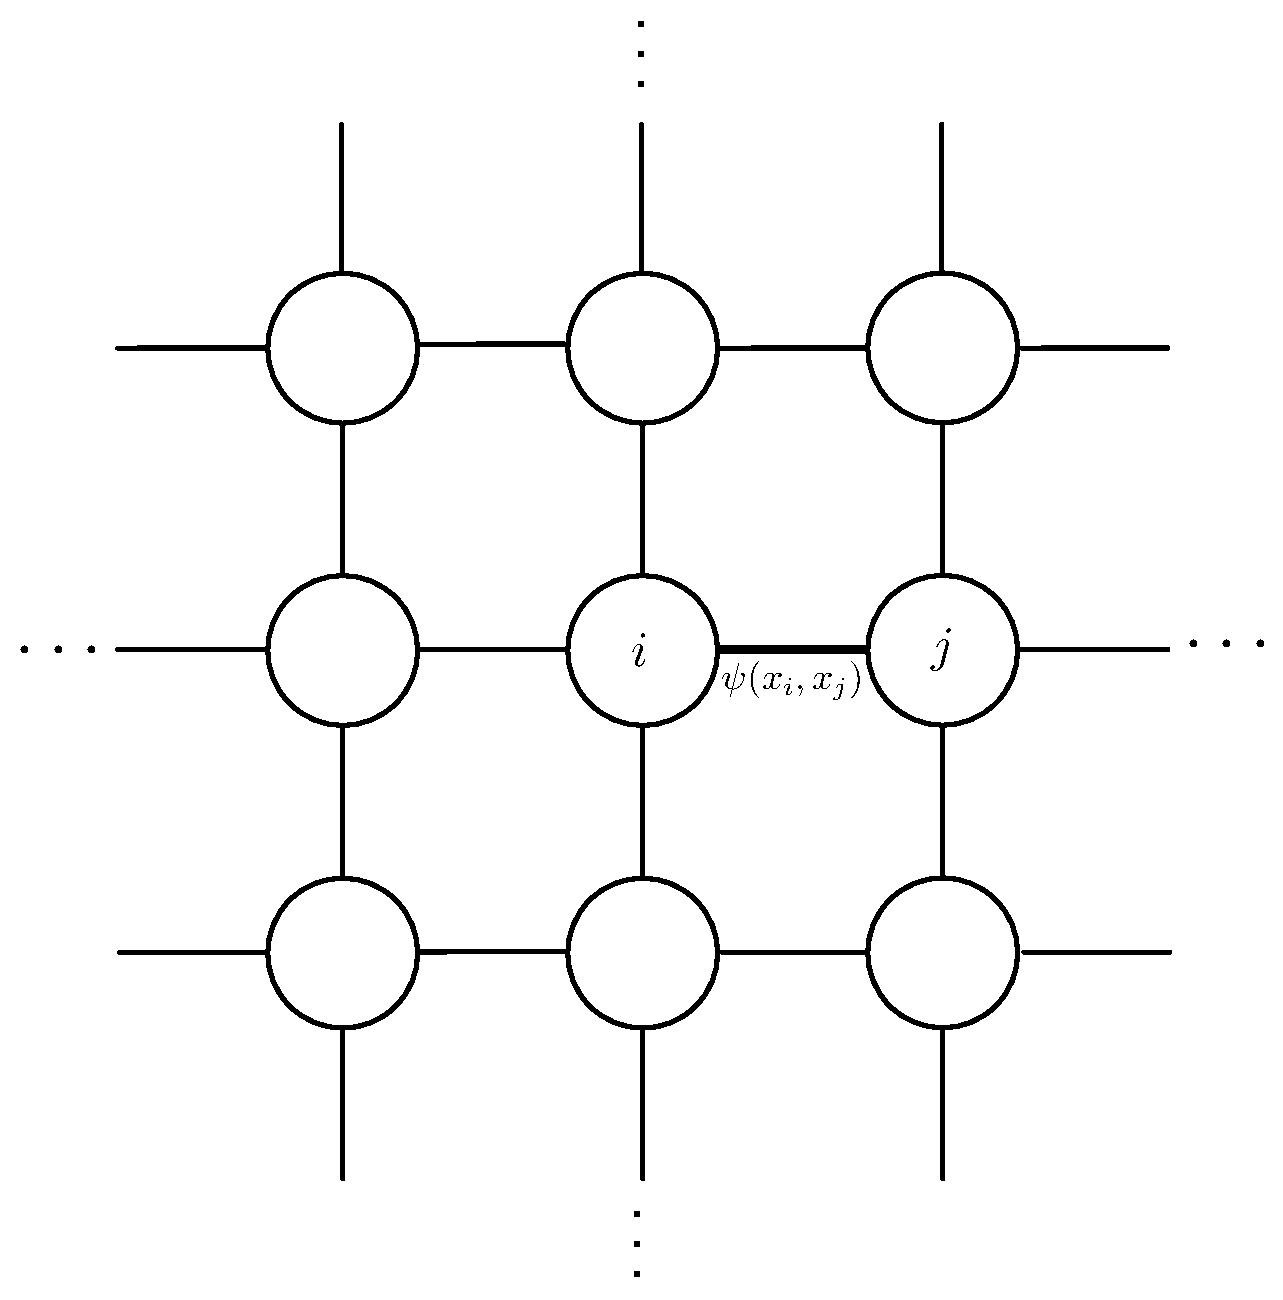
\includegraphics[width=3in]{figs/grid-mrf.pdf}
        \caption{Graphical model for the Ising model described in
            Equation~\ref{eq:ising}. Since this isn't a tree,
            we can't use the sum-pushing tricks of
            the belief propagation algorithm.}
        \label{fig:ising}
    \end{figure}
    Now suppose we also have a set of observations $\uY = \{Y_1,
        Y_2, \ldots, Y_n\}$, which we model as being conditionally independent
    given $\uX$:
    \begin{align}
        p_{\uY|\uX}(\uy|\ux) &= \prod_i p_{Y_i|X_i}(y_i|x_i) = \prod_i \phi(y_i, x_i),
    \end{align}
    where the conditional distribution $\phi$ is the same at every pixel. So,
    the full joint distribution over $\uX$ and $\uY$ is:
    \begin{align}
        p_{\uX, \uY}(\ux, \uy) 
        &= \frac{1}{Z} \cdot
           \prod_{(i,j) \in E} \psi(x_i, x_j) \cdot
           \prod_i \phi(y_i, x_i)
    \end{align}
    This is similar to a 2-D version of the HMM: we have random variables
    $\uX$ which are hidden and locally dependent, and observations $\uY$
    which are conditionally independent given $\uX$. Unlike the HMM,
    however, since the graphical model corresponding to this distribution
    is not a tree, we can't use techniques like the sum-product algorithm or
    the forward-backward algorithm like we can for trees or HMMs, respectively.
    \subsection{Exact inference is hard}
    Suppose we observe $\uY$ and wish to compute the posterior distribution over
    $\uX$:
    \begin{align}
        p_{\uX | \uY}(\uX | \uY) &= \frac{p_{\uX, \uY}(\ux, \uy)}{\sum_{\ux} p_{\uX, \uY}(\ux, \uy)}
    \end{align}
    Unfortunately, the sum in the denominator is over all $2^n$ possible
    configurations for $\ux$ (and because the graph isn't a tree, we can't
    use any of the sum-pushing tricks that are useful for the sum-product
    algorithm). So, computing the denominator is intractable. Computing the
    marginal distribution at any one pixel involves a similar summation in the
    numerator, and is also intractable. For example, a typical smartphone
    camera has 8 megapixels, or $8\times 10^6$ pixels, forcing us to sum over
    $2^{8\times 10^6}$ possibilities. As a comparison, the number of atoms in
    the universe is estimated to be about $2^{265}$!

    \paragraph{What about MAP estimation?}
    \begin{align}
        \argmax_\ux p_{\ux | \uY}(\ux | \uY) 
        &= \argmax_\ux p_{\uX, \uY}(\ux, \uy) \\
        &= \argmax_\ux 
            \left[\prod_{(i,j) \in E} \psi(x_i, x_j) \cdot
            \prod_i \phi(y_i, x_i)\right] 
    \end{align}
    Even though we eliminated the need to compute any intractable sums, we're
    still stuck: this is a maximization over $2^n$ discrete values, which we
    can't use any shortcuts for. So, doing exact inference requires us to search
    over every one of them, and so is
    intractable. In the next section, we'll look at a few ways for
    approximating this and other complex distributions.

    As mentioned before, it's important to note that this is not the only
    distribution for which inference is intractable, and the approximate
    methods discussed here are not the only approximations that we can use.

    \section{Approximate Inference: Sampling}
    In \emph{Monte Carlo} methods, we use randomly generated samples $x$ to
    approximate a quantity or distribution of interest, which we'll call $p_X$.
    In \emph{Markov Chain Monte Carlo (MCMC)} methods, these samples are
    generated ``Markov-chain style'': we start with a sample, which we use to
    generate the next sample, and so on. Each sample only depends on the one
    before it, and the transitions between samples are constructed so that in
    steady-state (i.e., after repeating many times), the samples we obtain come
    from $p_X$.
    \subsection{Metropolis-Hastings}
    The Metropolis-Hastings algorithm requires only two things:
    \begin{enumerate}
        \item The ability to compute unnormalized probabilities of samples
            $\tilde{p}_X(x)$: here, unnormalized is okay because we'll only be
            interested in ratios
        \item A proposal distribution $V(x^\prime|x)$, which tells us how to
            generate the next sample $x^\prime$ given the current sample $x$
    \end{enumerate}
    The algorithm itself is simple:

    \noindent
    \hrulefill
        \begin{algorithmic}[1]
            \Require{Unnormalized probability distribution $\tp_X(\cdot)$,
                     proposal distribution $V(\cdot | \cdot)$}
            \Statex
            \Function{MetropolisHastings}{$\tp_X, V$}
                \State{$x \gets $any valid value}
                \Loop
                    \State{$x^\prime \gets $Sample from $V(\cdot|x)$}
                    \State{$a \gets \min \left\{ 1, \frac{\tp_X(x^\prime)}{\tp_X(x)} \cdot \frac{V(x|x^\prime)}{V(x^\prime|x)}\right\}$} \label{line:mh-ratio}
                    \State{With probability $a$, $x \gets x^\prime$}
                    \State{Save $x$}
                \EndLoop
            \EndFunction
        \end{algorithmic}
    \hrulefill

    Often, we'll choose proposal distributions that are symmetric (i.e.,
    $V(x^\prime|x) = V(x|x^\prime)$), and the ratio in line~\ref{line:mh-ratio}
    reduces to $\tp_X(x^\prime)/\tp_X(x)$.  That is, if the new sample is more
    probable, we definitely accept it (the min is there just to avoid
    probabilities that are greater than 1), and if it is less probable, we
    randomly accept it depending on how much less probable it is. In general,
    we need to weight that ratio to make sure our proposal distribution isn't
    unfairly pushing us one way or the other: that's what the
    $V(x|x^\prime)/V(x^\prime|x)$ term is for.

    Some important points to note:
    \begin{enumerate}[(a)]
        \item Choosing a good proposal distribution can be tricky, and is
            usually problem-dependent. Suppose $X$ takes on values in between 0
            and 1000. Let's look at three different proposal distributions:
            \begin{itemize}
                \item $V_1(\cdot | x)$ is uniform over the interval $x \pm 50000$.
                \item $V_2(\cdot | x)$ is uniform over the interval $x \pm 1$.
                \item $V_3(\cdot | x)$ is uniform over the interval $x \pm 300$.
            \end{itemize}
            Most of the time, proposals generated from $V_1$ will be outside
            the range $[0,1000]$, and our acceptance probability will be 0.
            Proposals from $V_2$ will almost always be accepted, but it will
            take tens of thousands of iterations just to cover the entire
            space of possibilities. $V_3$ attempts to strike a balance in
            between these, with not too many rejections but a decent coverage
            of the sample space.
        \item Notice that we initialized completely arbitrarily: in many cases,
            this initialization could be in a particularly low-probability
            location. A common practice is to wait $K$ iterations before
            collecting any samples, to avoid any artifacts from initialization.
            In this case, $K$ is known as the \textbf{burn-in time}.
        \item Another somewhat common practice is to not save every single
            sample, but rather to wait a fixed number of iterations between
            each save. This prevents samples from being dependent on each
            other, but is not necessarily a problem for a well-chosen proposal
            distribution with enough samples.
    \end{enumerate}

    \subsubsection{Metropolis-Hastings MCMC for the Ising model}
    Let's return to the Ising model. Suppose for our proposal distribution
    $V(\cdot|\ux)$, we flip one randomly chosen value from $\ux$ (call it
    $x_k$), and use a distribution that is uniform over all such configurations.
    An example for a four-pixel image is shown in Figure~\ref{fig:proposal}.

    \begin{figure}
        \centering
        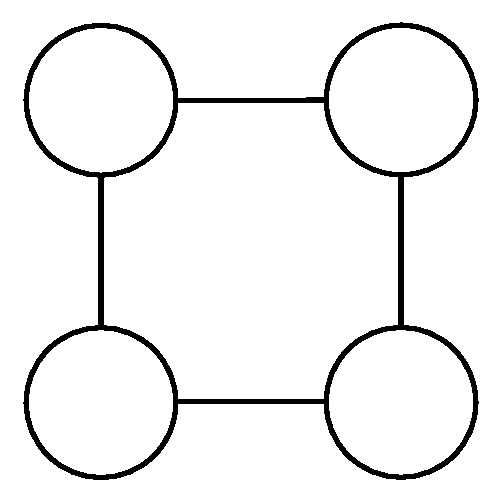
\includegraphics[width=1.5in]{figs/grid-mrf-small.pdf}
        \quad
        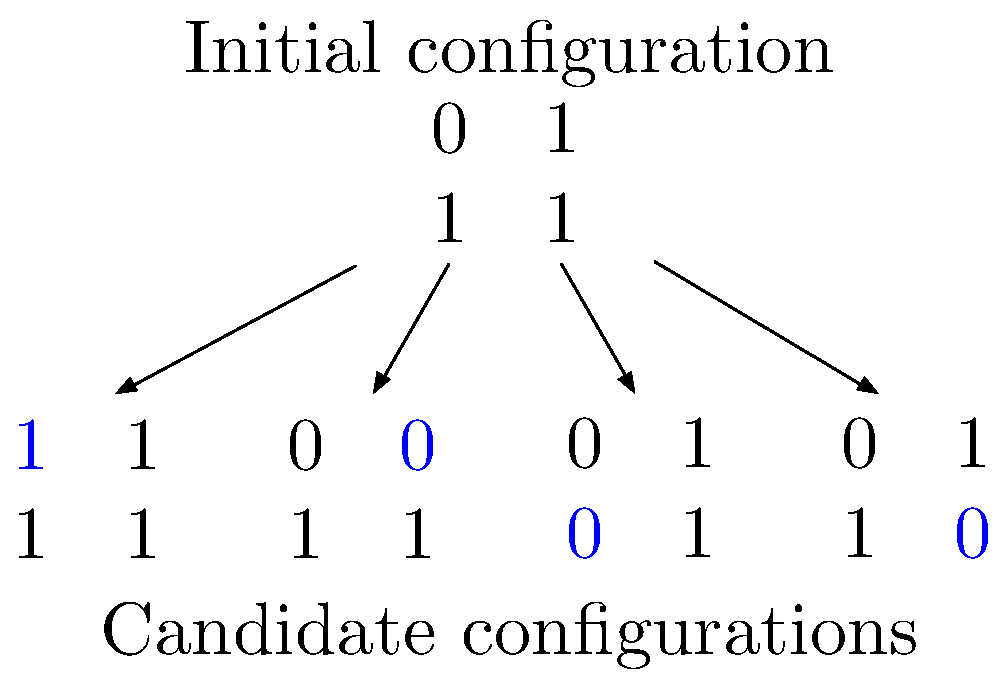
\includegraphics[width=3in]{figs/proposal-distribution.pdf}
        \caption{Example proposal distribution for a 4-pixel grid (left). The proposal
            distribution is uniform over the 4 candidates shown (right).}
        \label{fig:proposal}
    \end{figure}
    \noindent \textbf{Exercise}: Compute the acceptance probability for flipping $X_k$ from
    $x_k$ to $x_k^\prime$.

    \noindent \textbf{Solution}: We simply compute the ratio from line~\ref{line:mh-ratio}
    of the algorithm. We begin by noting that
    $V(\ux^\prime|\ux)=V(\ux|\ux^\prime)$, since $V$ flips $x_k$ with probability
    $1/n$ from either $\ux^\prime$ or $\ux$. So, we need only compute the ratio
    \begin{align*}
        \frac{\tp_\uX(\ux^\prime)}{\tp_\uX(\ux)} 
        &= \prod_{j: (j,k) \in E} \frac{\psi(x_j,x_k^\prime)}{\psi(x_j, x_k)} \cdot \frac{\phi(y_k, x_k^\prime)}{\phi(y_k, x_k)},
    \end{align*}
    since all terms not involving $x_k$ stay the same and therefore cancel
    between the numerator and the denominator. Therefore, for any proposed
    sample, we need only evaluate about 10 numbers and perform a few divisions
    and multiplications.

    \noindent \textbf{Exercise}: Why might this not be a good proposal distribution?
    Can you come up with a better one?

    \subsection{Gibbs Sampling}
    Like Metropolis-Hastings, Gibbs sampling is a flavor of MCMC, but it's
    conceptually simpler! If we want to sample from a distribution over several
    random variables, Gibbs sampling fixes all but one random variable, samples
    that one conditioned on the others, and then repeats the process for each
    random variable. So, all we need are the conditional distributions.

    We'll use the notation $\uX_{\neg i}$ to represent all of $\uX$ except $X_i$:
    for example,
    \begin{align*}
        \uX_{\neg 3} = \{X_1, X_2, X_4, X_5, X_6, \ldots, X_n\}.
    \end{align*}
    Then our algorithm is as follows:

    \noindent
    \hrulefill
    \begin{algorithmic}[1]
        \Require{Conditional distributions $p_{X_i|\uX_{\neg i}}(x_i | \ux_{\neg i})$}
        \Statex
        \Function{GibbsSample}{$p_{X_i|\uX_{\neg i}}(x_i | \ux_{\neg i})$}
            \State{$\ux \gets $any valid value}
            \Loop
                \For{$i$ in $\{1, \ldots, n\}$}
                    \State{$x_i \gets$Sample from $p_{X_i|\uX_{\neg i}}(\cdot|\ux_{\neg i})$}
                \EndFor
                \State{Save $\ux$}
            \EndLoop
        \EndFunction
    \end{algorithmic}
    \hrulefill

    As with Metropolis-Hastings MCMC, we often only start saving after a burn-in
    period, and sometimes will wait for several iterations of the outer
    loop between saves.

    \subsubsection{Gibbs sampling for the Ising Model}
    Let's return once again to the Ising model and look at how to apply Gibbs
    sampling there.

    \noindent \textbf{Exercise}: Compute the conditional distribution
    $p_{X_i | \uX_{\neg i}, \uY}(x_i | \ux_{\neg i}, \uy)$ up to a constant
    of proportionality. Explain why we don't need to compute normalizing constants.

    \noindent \textbf{Solution}: As always, we compute the conditional distribution
    as the joint distribution over all $\uX$ (conditioned on $\uY$) divided
    by the marginal distribution of what we're conditioning on, $\uX_{\neg i}$ (conditioned
    on $\uY$):
    \begin{align}
        p_{X_i | \uX_{\neg i}, \uY}(x_i | \ux_{\neg i}, \uy)
        &= \frac{p_{\uX| \uY}(\ux| \uy)}{p_{\uX_{\neg i}| \uY}(\ux_{\neg i}| \uy)} \\
        &\propto \prod_{j: (i,j) \in E} \psi(x_i, x_j) \phi(y_i, x_i) \cdot f(\uX_{\neg i}),
    \end{align}
    where the second equality follows from the fact that most terms in the
    first expression do not depend on $x_i$, and are therefore strictly a
    normalizing constant. We can in fact show that most of these terms cancel,
    but that isn't even necessary here, since we can just compute the
    normalization constant by plugging in 0 and 1 and adding up the results.
    For example, if plugging in gives 10 and 20 respectively, then we know that
    the probabilities are $1/3$ and $2/3$, since they must add up to 1.
\end{document}

